\section{Symmetric abstractions}

Define symmetry. Motivate why we care. What problems cant we solve?

Insert some examples of NNs failing to do 'simple' things.
When we pick aneural archietucture, we have little idea of how it will generalise.
It would be nice if we could control this.
Especially powerful, would be the ability to encourage symmetric ???s.


\subsection{Complexity}

How hard is it to find symmetries?
First, what do we mean by a symmetry?

\begin{align}
x, y \in X : \exists G \cdot x \cap
\end{align}



\subsection{n-dimensional Cart pole}

So, how can we test a learners ability to detect symmetries and exploit them?
We propose a simple test, the n-dimensional cart pole.

Many people realise that this problem can be reduce to $n$, one dimensional cart pole problems.
But the learner needs to infer that.

\cite{Brockman2016,baselines}

Why is this problem hard? The more dimensions there are, the more ways there are to fail.
Especially with respect to how exploration is done. In a single dimension, ...
Maybe you correctly balanced the pole in all dimensions except one. To bad, you dont get any reward.

\begin{figure}
\centering
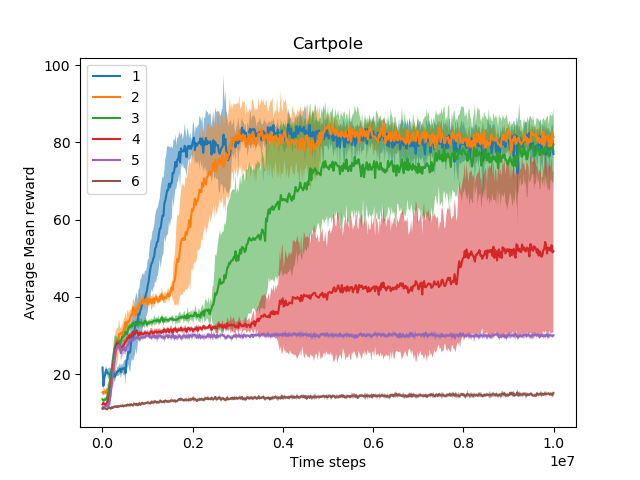
\includegraphics[width=1\textwidth,height=0.5\textheight]{../../pictures/figures/discrete-nd-cart.png}
\caption{PPO2 solving the nd cartpole problem with access to a \textit{Discrete} action space that grows with $2^N$.}
\end{figure}


\begin{figure}
\centering
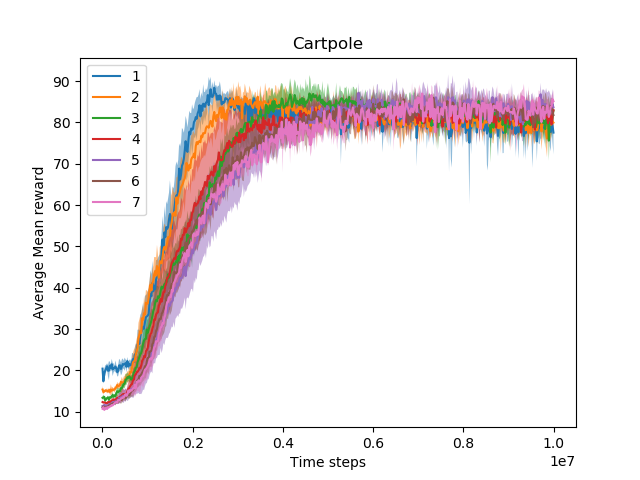
\includegraphics[width=1\textwidth,height=0.5\textheight]{../../pictures/figures/multibinary-nd-cart.png}
\caption{PPO2 solving the nd cartpole problem with access to a \textit{MultiBinary} action space that grows with $N$.}
\end{figure}

It seems surprising that access to the \textit{MultiBinary} action space provides such an advantage.
Also, it seems surprising that the an increase of 6 dimensions only results in approximately a ~2 million increase in the data required.
Is the learner doing some sort of intelligent sharing?
Why is it so hard for the Discrete learner? What operation does it find hard to learn. The ability to decode? $n$ bits to $2^n$ onehots?

Also, interesting to note that the 1D learner equipped with a \textit{Discrete}
action space achieves max performance at ~1.75 million samples, while the learner
equipped with a \textit{MultiBinary} action space achieves max performance at ~2.25 million samples. (significant??)

\section{No free lunches}

We want to


\subsection{Related work}

relationship to disentanglement.
As recently noted by \cite{Caselles-Dupre2019}, ...

A couple parts. Discovery of symmetries, explotation of the knowledge of symmetries.

Dicovery. Not much success.

Exploitation. Data augmentation, ...?


\subsection{Future work}

Formalise what we mean by 'simple'. Occam's razor. Compression, symmetry.
